\documentclass{beamer}
\mode<presentation>
\usetheme{CambridgeUS}
\usepackage[russian]{babel}
\usepackage[utf8]{inputenc}
\usepackage[T2A]{fontenc}
\usepackage{sansmathaccent}
\pdfmapfile{+sansmathaccent.map}
\title{Шумоподавление}
\author{Наумов Д.А.}
\date[12.03.2014] {Компьютерные музыкальные технологии и звуковой дизайн, 2014}

\begin{document}

%ТИТУЛЬНЫЙ СЛАЙД
\begin{frame}
  \titlepage
\end{frame}

%СОДЕРЖАНИЕ ЛЕКЦИИ
\begin{frame}
  \frametitle{Содержание лекции}
  \tableofcontents
\end{frame}

%РАЗДЕЛ 1
\section{Основные понятия}
\begin{frame}
Целью шумоподавления и восстановления звука является получение наилучшего звучания с минимальным вмешательством человека. По сути, редактирование исходной записи должно быть незаметным и не создавать новые артефакты, которые бы отвлекали слушателя.

Шумоподавление применяется, для того, чтобы:
\begin{itemize}
  \item улучшить восприятие сигнала, в том числе различимость речи;
  \item удалить искажения, наводки от сети электрического тока из записей музыки;
  \item упростить сведение мультитрековых композиций (например, уменьшив количество низкочастотных составляющих сигнала).
\end{itemize}

Иногда целей шумоподавления можно достичь в полном объеме, иногда приходится искать компромисс между уменьшением шумов и сохранением оригинального звучания.
\end{frame}

\begin{frame}
\textit{Шумом} может считаться любой нежелательный звук, присутствующий в аудио сигнале, например:
\begin{itemize}
\item шипение усилителя;
\item шум уличного движения;
\item наводки от сети переменного тока;
\item периодические щелчки на оцифрованной записи виниловой пластинки.
\end{itemize}

\textit{Искажение}~--– это нежелательное изменение формы сигнала. Примеры искажений:
\begin{itemize}
\item клипирование;
\item нелинейные искажения звукового сигнала, полученные при прохождении через усилитель c нелинейным коэффициентом передачи.
\end{itemize}
\end{frame}

\begin{frame}
  Пример спектрограммы сигнала с искажением:
  \centering{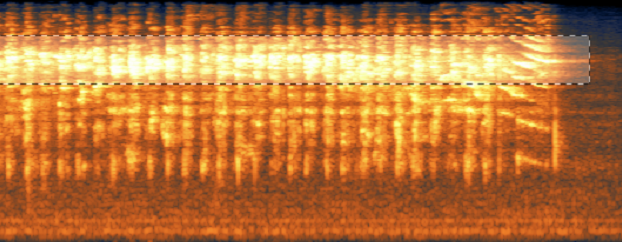
\includegraphics[width=0.95\textwidth]{pic-distort-01}}
\end{frame}


\begin{frame}
  \begin{itemize}
    \item \textbf{Шумоподавители} (\textit{Denoisers}) используются для того, чтобы уменьшить или полностью удалить постоянный фоновый шум. Это может быть фоновый шум помещения или шипение магнитофонной ленты (примеры "<случайных"> шумов), либо электрическое жужжание или гул от сети переменного тока (примеры "<тональных"> шумов). Шумоподавители могут быть одно- и многополосными, программными (\textit{Audition Noise Reduction}) и аппаратными (\textit{iZotope ANR-B}), общего применения или разработанными для особых задач, например, обработке вокала.
    \item \textbf{Инструменты удаления щелчков} (\textit{Declickers}) используются, чтобы уменьшить или удалить щелчки и хлопки. Причина их появления может быть разной: грязь и царапины на оцифровываемой виниловой пластинке,  скачки луча лазера при захвате данных с аудио компакт-диска, а также звуки причмокивания и размыкания губ.
  \end{itemize}
\end{frame}

\begin{frame}
  \begin{itemize}
    \item \textbf{Инструменты удаления треска} (\textit{Decracklers}) похожи на инструменты удаления щелчков, но оптимизированы для уменьшения или удаления более продолжительных и более тихих последовательных щелчков, которые, соединяясь воспринимаются нашим ухом как треск.
    \item \textbf{Инструменты удаления клипирования} (\textit{Declippers}) используются для восстановления артефактов цифрового и/или аналогового клипирования.
    \item \textbf{Инструменты удаления реверберации} (\emph{Dereverbs}) предназначены для удаления из сигнала нежелательной и отвлекающей реверберации. Эти инструменты полезны для коррекции диалогов, в том числе при \emph{ADR} (\emph{Automatic Dialog Replacement}~--- автоматическая замена диалога).
    \item \textbf{Инструменты визуального ручного редактирования сигнала} (\emph{Visual Editing Tools}) представляют собой комбинированные средства отображения и редактирования сигнала в различных формах: сигналлограммы и спектрограммы.
  \end{itemize}
\end{frame}

\begin{frame}
  В данной лекции будут рассмотрены следующие инструменты шумоподавления:
  \begin{itemize}
    \item стандартные инструменты подавления шума в \emph{Adobe Audition}, за исключением средств, которые представляют собой варианты фильтров, эквалайзеров и инструментов динамической обработки (они будут рассмотрены в соответствующих лекциях);
    \item некоторые средства из набора VST-инструментов, входящих в пакет \emph{Waves Restoration bundle};
    \item инструмент \emph{iZotope RX 3 Advanced}, который может использоваться и как VST-инструмент, и как отдельное приложение \emph{Win x86/x64};
  \end{itemize}
\end{frame}

\section{Устранение непериодических шумов}
\begin{frame}
Этапы шумоподавления непериодических шумов:
\begin{itemize}
  \item идентификация;
  \item выделение;
  \item применение нужного инструмента.
\end{itemize}

Трудности:
\begin{itemize}
  \item такие шумы могут вести себя непредсказуемо как по частоте, так и во времени;
  \item в отличие от нетональных шумов, гула, щелчков и треска, такие шумы нельзя удалить с использованием автоматических методов, а ручная коррекция может быть довольно трудоемкой;
  \item даже самые современные инструменты могут создать артефакты в сигнале в результате процесса шумоподавления;
  \item всегда существует множество разнообразных инструментов, подходящих для решения конкретной задачи по подавлению шума, а выбор наиболее эффективного средства тоже непростая задача.
\end{itemize}
\end{frame}

\subsection{Устранение непериодических шумов в Adobe Audition}
\begin{frame}
В \textit{Adobe Audition} в режиме отображения спектрограммы можно использовать следующие инструменты для того, чтобы выделить звук в определенном частотном диапазоне:
\begin{itemize}
\item \textit{Marquee Selection}~--– выделение прямоугольной области,
\item \textit{Lasso Selection}~--– выделение при помощи лассо,
\item \textit{Paintbrush Selection}~--– эффект кисти.
\end{itemize}
\centering{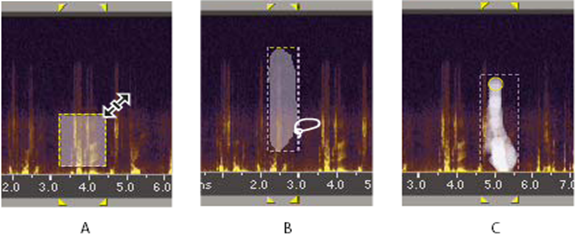
\includegraphics[width=0.75\textwidth]{pic-spectroedit-01}}
\end{frame}

\begin{frame}
Для быстрого исправления небольших дискретных искажений, таких как отдельные хлопки и щелчки, следует использовать инструмент \textit{Spot Healing Brush}:
\begin{itemize}
\item в режиме \textit{Spectral Frequency Display} выбрать инструмент \textit{Spot Healing Brush};
\item на панели инструментов установить размер кисти (\textit{Brush Si}ze).
\item в главном окне щелкнуть или провести мышью по области искажения.
\end{itemize}
\centering{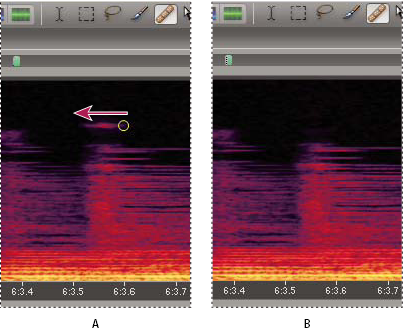
\includegraphics[width=0.5\textwidth]{pic-spectroedit-02}}
\end{frame}

\subsection{Устранение непериодических шумов в iZotope~RX~3}
\begin{frame}
Инструмент \emph{iZotope~RX~3}~--- это полноценный инструмент для проведения шумоподавления и восстановления звука, который может использоваться и как VST-инструмент, и как отдельное приложение \emph{Win x86/x64}.

~

Основные инструменты и их возможности в \emph{iZotope~RX~3}:
\begin{itemize}
  \item \emph{Denoise, Remove Hum}~--- удаление фонового шума и шумов и искажений сигнала, в том числе шипение, гул и жужжание;
  \item \emph{Spectral Repair}~---замена поврежденных или отсутствующих фрагментов сигнала с использованием шаблонов на основе естественных звуков;
  \item \emph{DeClick, DeCrackle}~--- удаление щелчков, хлопков;
  \item \emph{DeClip}~---избавление от клипирования.
\end{itemize}
\end{frame}

\begin{frame}
\centering{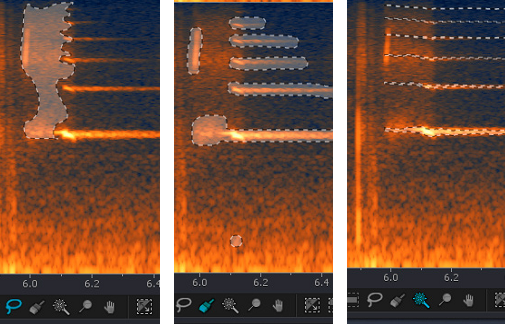
\includegraphics[width=0.5\textwidth]{pic-spectroedit-03}}
\begin{itemize}
  \item \emph{Time Selection}~--- выделение временного интервала;
  \item \emph{Time-Frequency Selection}~--- выделение прямоугольного фрагмента;
  \item \emph{Frequency Selection}~--- выделение диапазона частот;
  \item \emph{Lasso}~--- позволяет нарисовать произвольный замкнутый контур.
  \item \emph{Brush}~--- выделение "<кистью">;
  \item \emph{Magic Wand}~--- "<волшебная палочка">, автоматическое "<умное"> выделение некоторого диапазона.
\end{itemize}
\end{frame}

\begin{frame}
\begin{itemize}
  \item \emph{Attenuate} (ослабление)~--- в этом режиме звук в выделенном фрагменте заменяется звуками, расположенными в близлежащих областях.
  \item \emph{Pattern} (шаблон)~--- в данном режиме ищется наиболее подходящий фрагмент сигнала, которым и заменяется выделенный фрагмент.
  \item \emph{Partials + Noise}~--- это более сложный вариант режима \emph{Pattern}, выполняющий более точную интерполяцию в тех случаях, когда происходит изменение высоты тона, в том числе в виде вибрато.
\end{itemize}
\centering{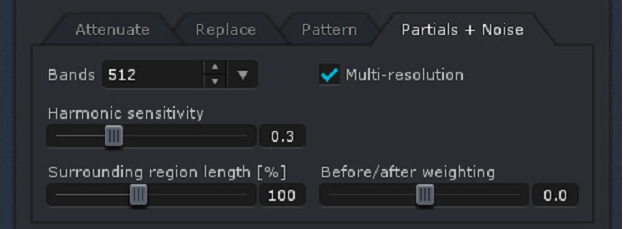
\includegraphics[width=0.5\textwidth]{pic-repair-01}}
\end{frame}

\begin{frame}
\begin{itemize}
  \item \emph{Replace} (замена)~--- данный режим используется для замены поврежденных фрагментов тонального сигнала.
\end{itemize}
\centering{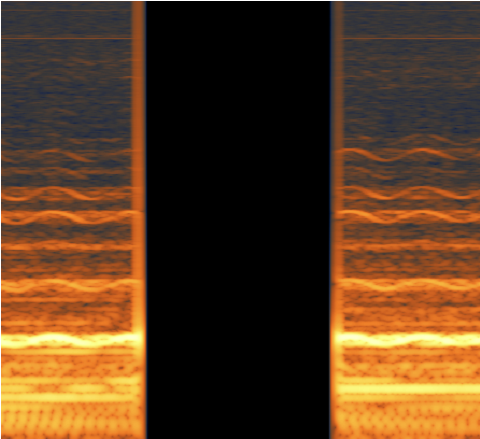
\includegraphics[width=0.5\textwidth]{pic-repair-02}}
\end{frame}

\section{Устранение нетональных шумов}
\begin{frame}
Для удаления нетональных шумов необходимо иметь информацию о шуме: чем больше статистических свойств шума известно, тем эффективнее процесс шумоподавления.

Информацию о шуме можно получить, анализируя спектр фрагмента волновой формы, содержащий только шумы (шипение микрофона, фоновые звуки и т. п.). При выполнении процесса шумоподавления будет считаться, что выбранный фрагмент содержит только шум.

\centering{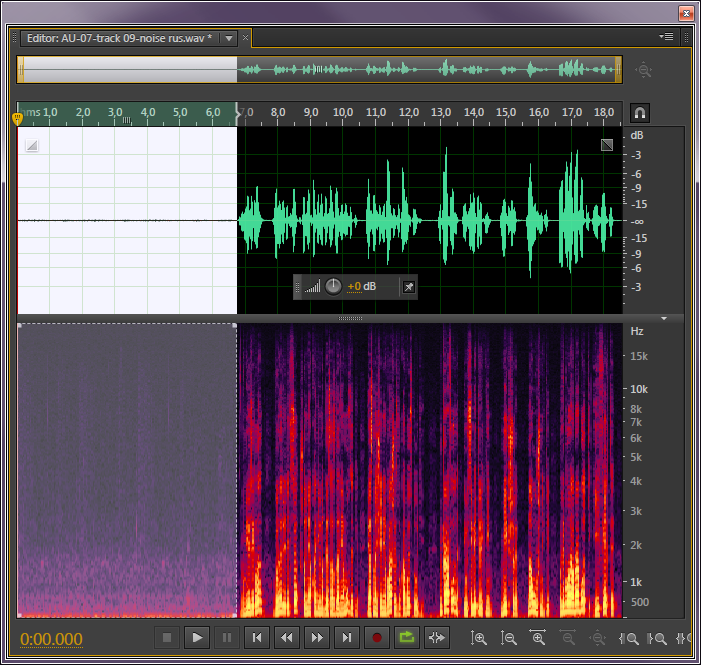
\includegraphics[width=0.5\textwidth]{pic-noisereduction-01}}
\end{frame}

\subsection{Устранение нетональных шумов в Adobe Audition}
\begin{frame}
Рассмотрим процесс шумоподавления при помощи инструмента \textit{Noise Reduction}.
\begin{itemize}
    \item выделить фрагмент волновой формы без полезной информации, но содержащий характерный для этой волновой формы шум
    \item выполнить команду \textit{Effects > Restoration > Noise Reduction}. В открывшемся окне нажать кнопку "<\emph{Capture Noise Print}">. 
    \item На координатном поле отображаются три графика:        \centering{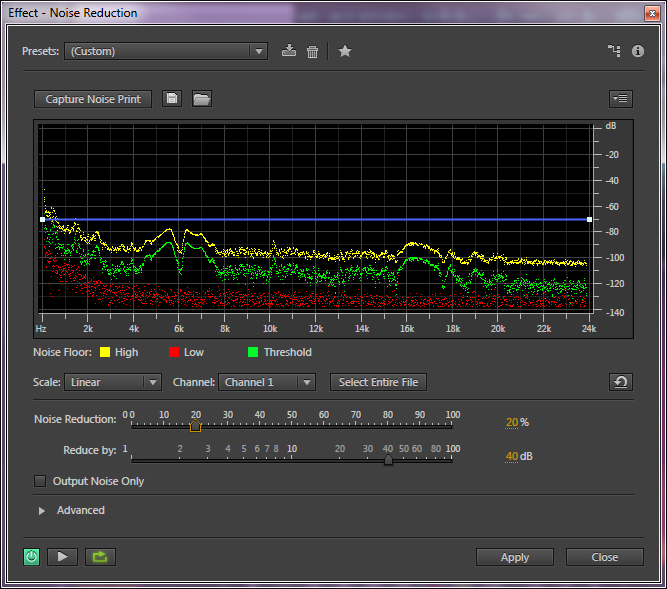
\includegraphics[width=0.5\textwidth]{pic-noisereduction-02}}
\end{itemize}
\end{frame}


\begin{frame}
\begin{itemize}
    \item Снять флаг \textit{Output Noise Only} (выводить только шум), если он был установлен. Нажать на кнопку "\textit{Preview Play/Stop}". Прослушивая фрагмент с шумом, установить значение параметра \textit{Noise Reduction}, при котором шум становится практически не слышен (абсолютной тишины добиваться не следует). Если выбрать порог подавления слишком высоким, то улучшения субъективного ощущения тишины в паузах не будет, зато в сигнале появятся искажения в виде металлического призвука.
    \item Установить флаг \textit{Output Noise Only}. Прослушивая звук и уменьшая значение \textit{Noise Reduction}, добиться, чтобы не удалялись полезные составляющие звука (то есть при прослушивании не были бы слышны отдельные гласные, согласные звуки и т.п.).
    \item Установить компромиссное значение параметра \textit{Noise Reduction}, чтобы, с одной стороны, обеспечивать достаточный уровень шумоподавления, а с другой~--– не затрагивать полезный сигнал.
\end{itemize}
\end{frame}

\subsection{Waves X-Noise и Z-Noise}
\begin{frame}
Инструмент \emph{Waves X-Noise} также предназначен для удаления фонового шума. 

~

В отличие от инструмента \textit{Adobe Audition Noise Reduction}, инструмент \emph{X-Noise} может быть использован в режиме реального времени после предварительной настройки профиля шума.

\centering{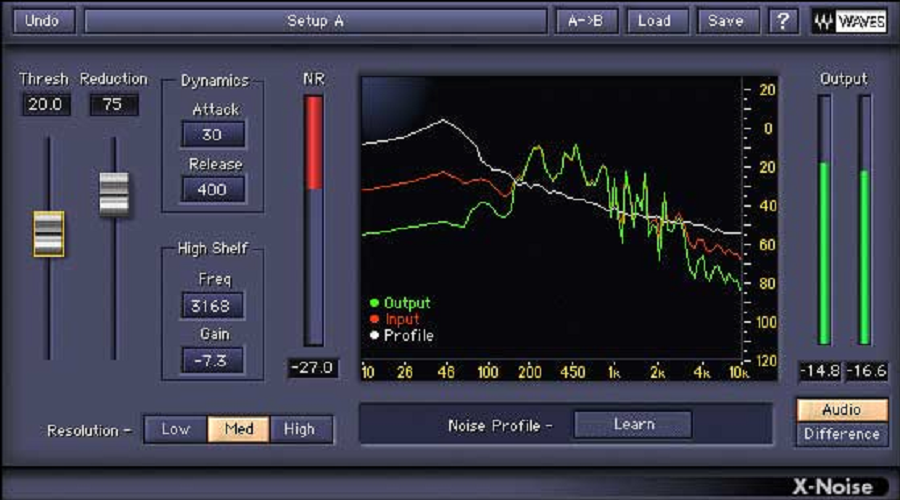
\includegraphics[width=0.5\textwidth]{pic-xnoise-01}}
\end{frame}

\begin{frame}
Инструмент \emph{Waves Z-Noise} отличается от \emph{Waves X-Noise} возможностью более точной настройки профиля шума. 

~

В распоряжении пользователя имеется пятиполосный параметрический эквалайзер, позволяющий вручную корректировать профиль шума.

\centering{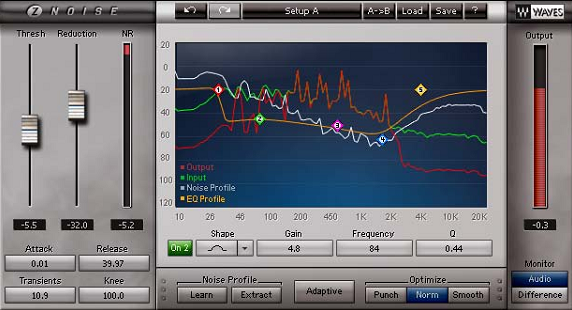
\includegraphics[width=0.5\textwidth]{pic-znoise-01}}
\end{frame}

\subsection{Устранение нетональных шумов в iZotope RX3 Denoise}
\begin{frame}
Инструмент \emph{iZotope Denoise} также предназначен для шумоподавления на основе профиля шума. Рассмотрим отличия данного инструмента от ранее описанных:
\begin{itemize}
  \item возможность выделения не связанных областей для получения профиля шума;
  \item возможность раздельного управления уровнем подавления случайных и тональных шумов (\emph{Noisy, Tonal Reduction});
  \item возможность управления качеством обработки (параметр \emph{Quality}) и уровнем вносимых искажений (параметр \emph{Artifact Control}).
\end{itemize}

\centering{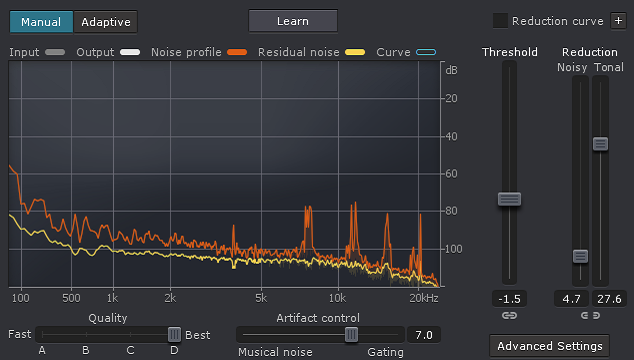
\includegraphics[width=0.5\textwidth]{pic-rx3denoise-01}}
\end{frame}


\section{Устранение щелчков и треска}
\begin{frame}
Щелчки и хлопки могут оказаться в записи сигнала на любой стадии его обработки. Рассмотрим различные причины их возникновения:
\begin{itemize}
  \item цифровые ошибки, которые создают быстрые резкие перепады в амплитуде сигнале;
  \item ошибки, возникшие из-за повреждения носителя аналогового сигнала (как правило, это более длительные искажения по сравнению с цифровыми);
  \item статическое электричество;
  \item касание микрофона по неосторожности;
  \item плохой контакт соединительных кабелей;
  \item помехи от электрической сети;
  \item звуки размыкания губ и т.д.
\end{itemize}
\end{frame}

\begin{frame}
Для того чтобы найти щелчки на волновой форме, следует переключиться в режим отображения \textit{Spectral Frequency Display}. Большинство щелчков будут видны как вертикальные линии, яркие на всей полосе частот.
\centering{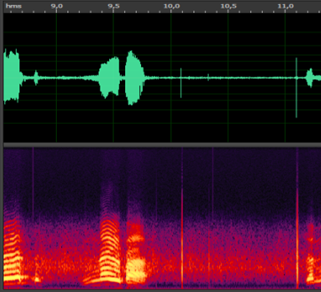
\includegraphics[width=0.5\textwidth]{pic-click-01}}
\end{frame}

\begin{frame}
Пример спектрограммы сигнала с щелчками
\centering{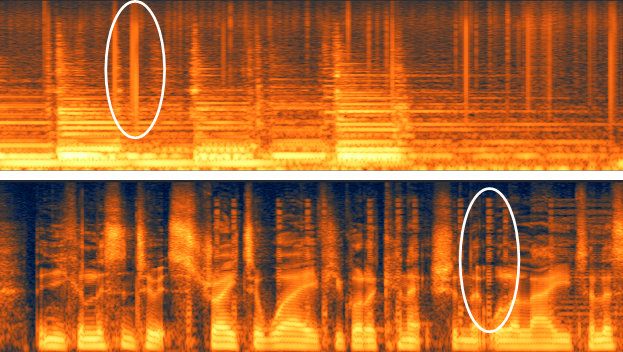
\includegraphics[width=0.5\textwidth]{pic-click-05}}

~

Пример спектрограммы сигнала с помехами от сотового телефона
\centering{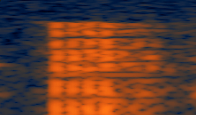
\includegraphics[width=0.35\textwidth]{pic-click-06}}
\end{frame}

\subsection{Adobe Audition > DeClicker}
\begin{frame}
Средства \textit{Diagnostics > DeClicker} и \textit{Noise Reduction \& Restoration > Automatic Click Remover} позволяют определить и удалить такие искажения, как щелчки и хлопки.

~

Рассмотрим параметры эффекта \textit{Automatic Click Remover}.

\centering{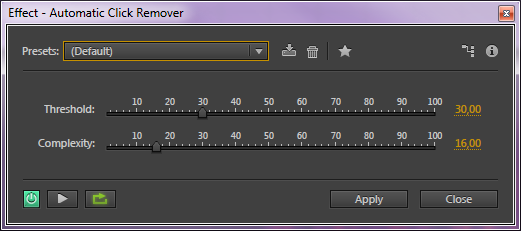
\includegraphics[width=0.5\textwidth]{pic-click-02}}
\end{frame}

\begin{frame}
Окно эффекта \textit{Diagnostics > DeClicker}
\centering{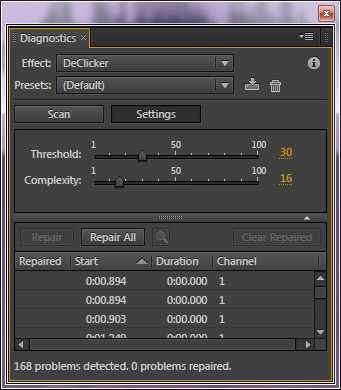
\includegraphics[width=0.5\textwidth]{pic-click-03}}
\end{frame}

\subsection{Waves > X-Click}
\begin{frame}
Инструмент \emph{X-Click} позволяет эффективно устранять щелчки старых виниловых пластинок и при правильном применении не создает дополнительных артефактов~--- искажений, вносимых эффектом. Инструмент \emph{X-Click} имеет два параметра настройки для идентификации щелчков:
\begin{itemize}
  \item Параметр \textbf{порог} (\textit{Threshold}) задает амплитуду искомых щелчков. 
  \item Параметр \textbf{форма} (\textit{Shape}) задает количество отсчетов в одном щелчке. 
\end{itemize}

\centering{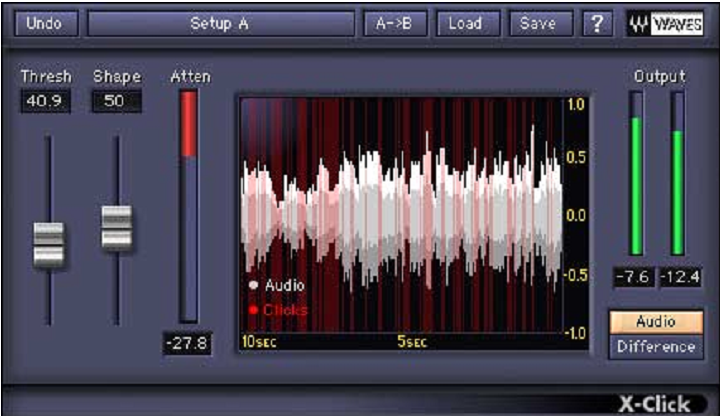
\includegraphics[width=0.5\textwidth]{pic-click-04}}
\end{frame}

\subsection{Waves > X-Crackle}
\begin{frame}
\textbf{Треск} (\emph{Crackle})~--- небольшие по амплитуде, короткие по длительности (несколько отсчетов) щелчки или хлопки, в большом количестве присутствующие в сигнале. Щелчки выражены более явно, чем треск, и часто имеют большую амплитуду, чем полезный сигнал. 

\begin{itemize}
  \item \textbf{Порог} (\emph{Threshold}) определяет амплитуду звука, который будет идентифицироваться как треск. 
  \item \textbf{Ослабление} (\emph{Reduction}) задает, на сколько децибел будут ослаблен обнаруженный треск.
\end{itemize}

\centering{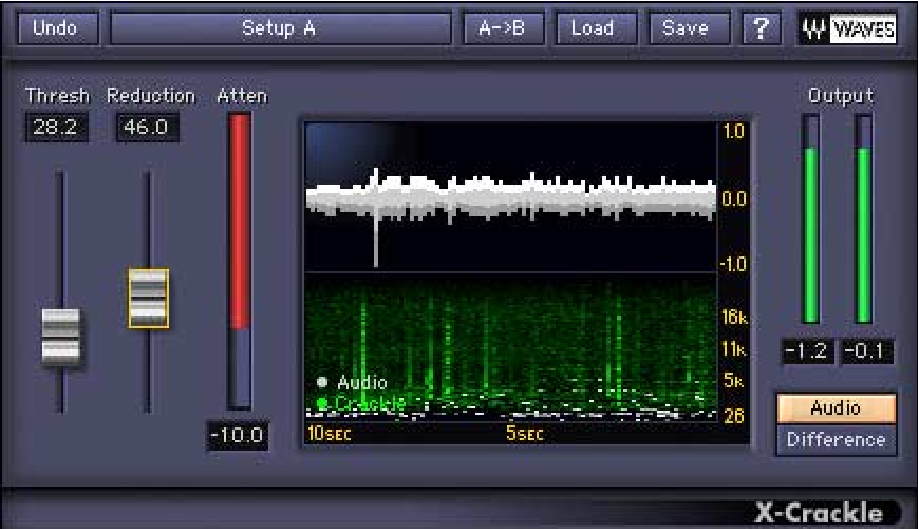
\includegraphics[width=0.5\textwidth]{pic-crackle-01}}
\end{frame}


\subsection{iZotope Ozone > Declick \& Decrackle}
\begin{frame}
Инструмент \emph{Declick} полезен при восстановлении звука оцифрованных виниловых пластинок, избавления от таких шумов, как щелчки, хлопки и треск. Как правило, длительность отдельного щелчка не превышает 10 миллисекунд. Инструмент \emph{Decrackle} предназначен для удаления более длительных помех в сигнале, воспринимаемые нами как слабый треск.

\centering{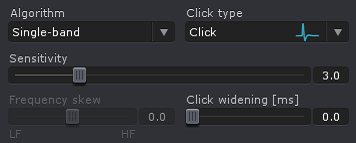
\includegraphics[width=0.5\textwidth]{pic-rx3declick-03}}

\centering{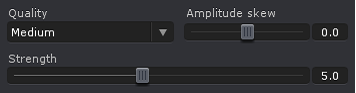
\includegraphics[width=0.5\textwidth]{pic-rx3decrackle-01}}
\end{frame}

\begin{frame}
Для удаление щелчков и треска необходимо выполнить следующие шаги.
\begin{enumerate}
  \item Выберите нужное значение параметра \emph{Algorithm} для модуля \emph{Declick}:
  \begin{itemize}
    \item Режим \emph{Single-band} хорошо работает с очень короткими "<цифровыми"> щелчками.
    \item Ремим \emph{M-band} (\emph{multi-band}) предназначен для более длительных "<аналоговых"> щелчков.
  \end{itemize}
  \item Воспроизведите сигнал.
  \item Во время воспроизведения настройте параметр \emph{Declick Sensitivity}, задающий чувствительность детектора щелчков или \emph{Decrackle Strength} для чувствительности детектора треска. Необходимо добиться того, что большинство щелчков будет удалено, при этом полезный сигнал не будет повреждаться.
  \item Для лучшего контроля за тем, какие звуки идентифицируются как щелчки и треск, можно использовать переключатель \emph{Clicks/Crackle Only} во время воспроизведения сигнала,~--- это позволит  услышать, какие звуки будут удалены из сигнала.
\end{enumerate}
\end{frame}

\begin{frame}
Спектрограмма до и после удаления щелчков

\centering{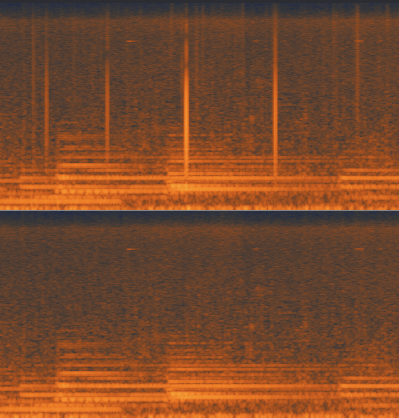
\includegraphics[width=0.5\textwidth]{pic-rx3declick-01}}
\end{frame}

\begin{frame}
Спектрограмма до и после удаления треска

\centering{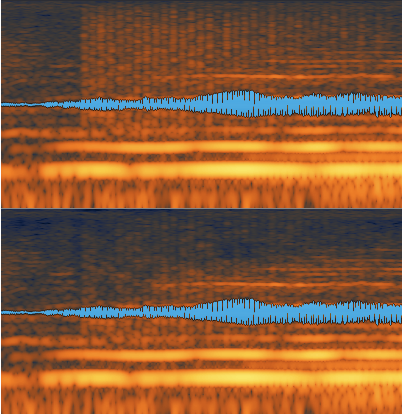
\includegraphics[width=0.5\textwidth]{pic-rx3declick-02}}
\end{frame}


\section{Устранение клипирования}
\begin{frame}
\textit{Клипирование}~--- это искажение, возникающее из-за неправильной регулировки уровня записываемого сигнала или из-за его случайного увеличения во время записи, приведшее к переполнению разрядной сетки аналого-цифрового преобразователя.

~

\centering{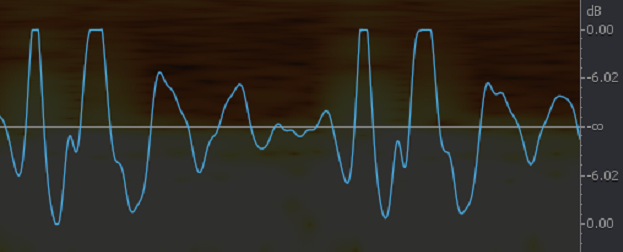
\includegraphics[width=0.5\textwidth]{pic-clip-01}}
\end{frame}

\begin{frame}
Целью удаления клипирования является восстановление клипированых фрагментов сигнала таким образом, чтобы их звучание было бы наиболее близко к оригинальному. Нельзя избавиться от клипирования, просто уменьшив громкость: формально клипированных отсчетов не будет, но само искажение останется.

~

\centering{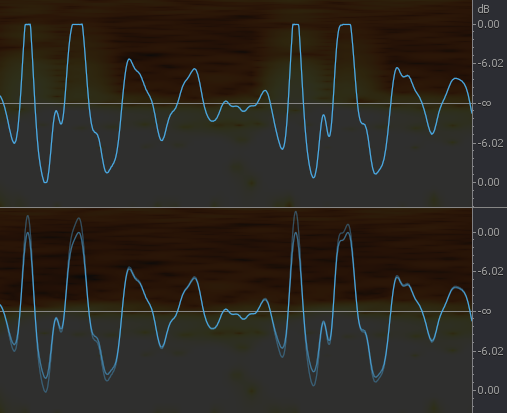
\includegraphics[width=0.5\textwidth]{pic-clip-02}}
\end{frame}


\subsection{Применение инструмента Adobe Audition DeClipper}
\begin{frame}
\textit{Adobe Audition DeClipper} вызывается командой \textit{Effects > Diagnostics > DeClipper}.

\centering{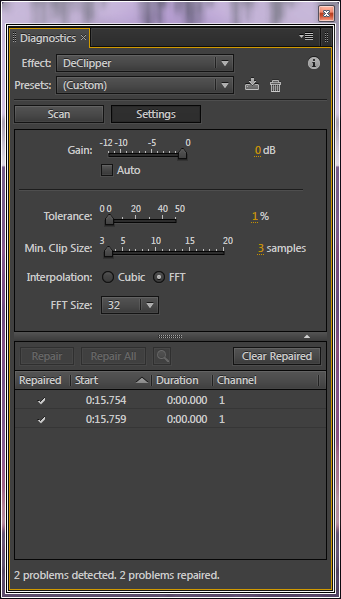
\includegraphics[width=0.3\textwidth]{pic-declipper-01}}

Алгоритм избавления от клипирования следующий:
\begin{itemize}
\item установить значение параметра \textit{Gain} вручную или установить флаг \textit{Auto};
\item нажать кнопку \textit{Scan};
\item нажать кнопку \textit{Repair All}.
\end{itemize}
\end{frame}

\subsection{Применение инструмента iZotope~RX~3 Declip}
\begin{frame}
Инструмент \emph{Declip} производит обработку части сигнала, которая окажется выше задаваемого порога, выполняя интерполяцию сигнала с целью получения более натуральной огибающей. Процесс работы с инструментом состоит из двух простых шагов:

\begin{itemize}
  \item поиск клипированных отсчетов;
  \item определение уровня клипированных отсчетов и выполнение обработки.
\end{itemize}

\centering{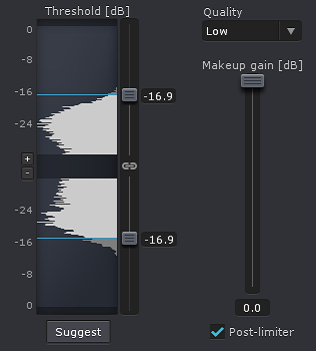
\includegraphics[width=0.4\textwidth]{pic-rx3declip-01}}
\end{frame}

\begin{frame}
Левую часть окна занимает гистограмма сигнала, при этом установить порог клипирования можно независимо для положительных и отрицательных значений отсчетов. Одним из признаков наличия клипирования является наличие максимумов на гистограмме на уровнях, близких к максимальному уровню сигнала:

\centering{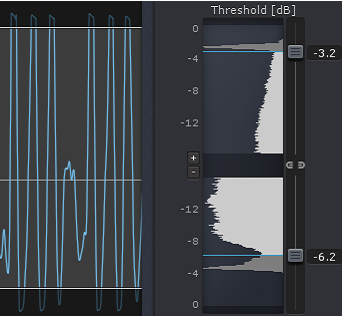
\includegraphics[width=0.4\textwidth]{pic-rx3declip-02}}
\end{frame}

\begin{frame}
Для устранения клипирования необходима настройка следующих параметров:
\begin{itemize}
  \item Threshold (dBFS); 
  \item Threshold Link; 
  \item кнопка Suggest;
  \item Quality;
  \item Makeup Gain (dB);
  \item Post-limiter;
\end{itemize}
\centering{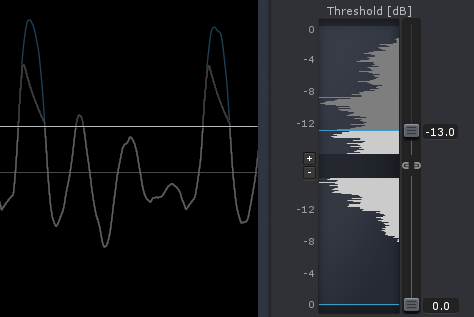
\includegraphics[width=0.4\textwidth]{pic-rx3declip-03}}
\end{frame}

\section[iZotope RX 3 Dereverb]{Устранение реверберации при помощи iZotope RX 3 Dereverb}
\begin{frame}
Инструмент \emph{Dereverb} позволяет задавать уменьшать уровень реверберации в сигнале. При помощи данного инструмента запись, сделанную в большом помещении с сильном эхо можно как бы превратить в запись, сделанную в обычной комнате, а запись в комнате~--- в запись в помещении со звукоизоляцией.

  \centering{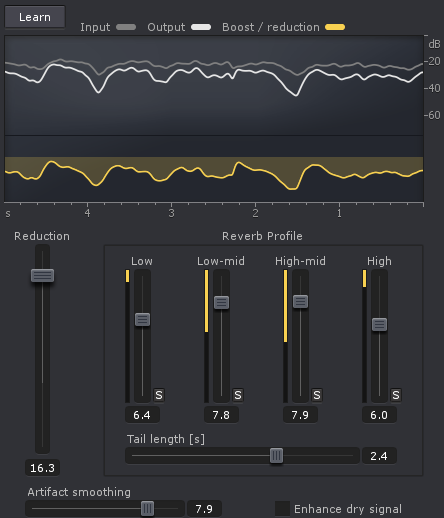
\includegraphics[width=0.4\textwidth]{pic-rx3dereverb-01}}
\end{frame}
\begin{frame}
Звук, записанный в помещении, можно разложить на две составляющих:
\begin{itemize}
  \item прямой звук;
  \item реверберационный хвост;
\end{itemize}

Уровень хвоста реверберации ослабляется с течением времени, причем скорость ослабления зависит от различных факторов, таких, как размер и материал стен помещения, его геометрия и т.д.

Инструмент \emph{Dereverb} выполняет обработку сигнала, изменяя соотношение обнаруженного прямого звука, и заданных (рассчитанных) параметров реверберации, таких как время ослабления сигнала на различных частотах.
\end{frame}
\begin{frame}
На спектрограмме наличие реверберации можно обнаружить по наличию некоторой размытости. 

\centering{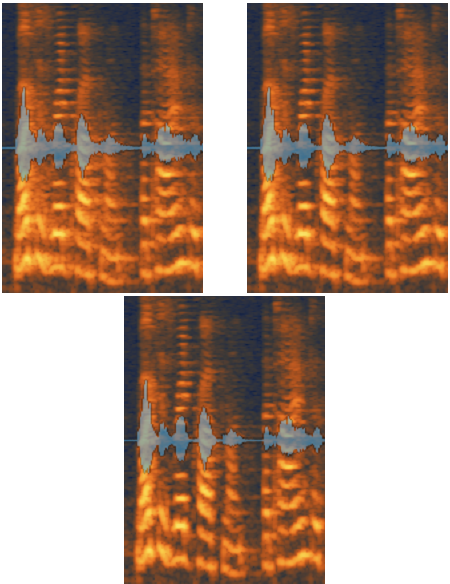
\includegraphics[width=0.5\textwidth]{pic-rx3dereverb-02}}
\end{frame}

\begin{frame}
Для того, чтобы приступить к уменьшению реверберации в сигнале, необходимо получить так называемый "<профиль реверберации">. Для этого необходимо выделить фрагмент сигнала, длительностью около 5 секунд, который будет содержать фоновый шум помещения в начале, полезный сигнал и хвост реверберации.

~

После получения профиля реверберации (после нажатия на кнопку \textit{Learn}) в верхней части окна отобразятся графики входного, выходного сигнала и величина ослабления (частотная характеристика профиля реверберации). 

~

Иногда хороших результатов удается достичь, применяя инструмент \emph{Dereverb} дважды.
\end{frame}

\section[Шумоподавление в записях диалогов]{Шумоподавление в записях диалогов при помощи iZotope RX 3 Dialog Denoiser}
\begin{frame}
Инструмент \emph{Dialogue Denoiser} позволяет осуществлять подавление шума в записях, в которых уровень шума значительно отличается от уровня полезного сигнала. Уровень шума задается при помощи графика порога шума. 

~

Если уровень сигнал ниже порога, то он считается шумом и будет подавляться, если выше ~--- полезным сигналом. Настройка формы графика порога шума осуществляется при помощи шести контрольных точек.
\centering{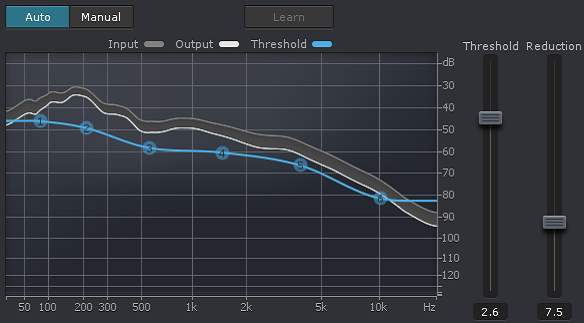
\includegraphics[width=0.4\textwidth]{pic-rx3dialog-01}}
\end{frame}
\end{document}
